\documentclass[12pt,a4paper]{article}
\usepackage{ctex}
\usepackage{amsmath,amscd,amsbsy,amssymb,latexsym,url,bm,amsthm}
\usepackage{epsfig,graphicx,subfigure}
\usepackage{enumerate}
\usepackage{wrapfig}
\usepackage{mathrsfs,euscript}
\usepackage[usenames]{xcolor}
\usepackage{hyperref}
\usepackage[vlined,ruled,linesnumbered]{algorithm2e}
\hypersetup{colorlinks=true,linkcolor=black}

\newtheorem{theorem}{Theorem}
\newtheorem{lemma}[theorem]{Lemma}
\newtheorem{proposition}[theorem]{Proposition}
\newtheorem{corollary}[theorem]{Corollary}
\newtheorem{exercise}{Exercise}
\newtheorem*{solution}{Solution}
\newtheorem*{conclusion}{Conclusion}
\newtheorem{definition}{Definition}
\theoremstyle{definition}

\renewcommand{\thefootnote}{\fnsymbol{footnote}}

\newcommand{\postscript}[2]
 {\setlength{\epsfxsize}{#2\hsize}
  \centerline{\epsfbox{#1}}}

\renewcommand{\baselinestretch}{1.0}

\setlength{\oddsidemargin}{-0.365in}
\setlength{\evensidemargin}{-0.365in}
\setlength{\topmargin}{-0.3in}
\setlength{\headheight}{0in}
\setlength{\headsep}{0in}
\setlength{\textheight}{10.1in}
\setlength{\textwidth}{7in}
\makeatletter \renewenvironment{proof}[1][Proof] {\par\pushQED{\qed}\normalfont\topsep6\p@\@plus6\p@\relax\trivlist\item[\hskip\labelsep\bfseries#1\@addpunct{.}]\ignorespaces}{\popQED\endtrivlist\@endpefalse} \makeatother
\makeatletter
\renewenvironment{solution}[1][Solution] {\par\pushQED{\qed}\normalfont\topsep6\p@\@plus6\p@\relax\trivlist\item[\hskip\labelsep\bfseries#1\@addpunct{.}]\ignorespaces}{\popQED\endtrivlist\@endpefalse} \makeatother

\begin{document}
\noindent

%========================================================================
\noindent\framebox[\linewidth]{\shortstack[c]{
\Large{\textbf{Homework 06}}\vspace{1mm}\\
CS499-Mathematical Foundations of Computer Science, Jie Li, Spring 2020.}}
\begin{center}
\footnotesize{\color{blue}Name: ������ (Hongjie Fang)  \quad Student ID: 518030910150 \quad Email: galaxies@sjtu.edu.cn}
\end{center}
\section{Warmup Problems}
\begin{enumerate}
  \item [1. ] What are the ${n \brack m} = 11$ permutations of $\{1,2,3,4\}$ that have exactly two cycles? (The cyclic forms appear in Formula (6.4) in textbook; non-cyclic forms like $2314$ are desired instead.)
  \begin{solution}
     Permutations $2314$, $2431$, $3241$, $1342$, $3124$, $4132$, $4213$, $1423$, $2143$, $3412$ and $4321$ all have exactly two cycles. Take $4132$ for instance, its two cycles are $[1,4,2]$ and $[3]$.
  \end{solution}

  \item [2. ] There are $m^n$ functions from a set of $n$ elements into a set of $m$ elements. How many of them range over exactly $k$ different function values?
  \begin{solution}
    According to the definition of Stirling's number, there are ${n \brace k}$ ways to divide $n$ elements into $k$ non-empty subset. We assume that the elements in every non-empty subset have the same function value, therefore, the total $n$ elements range over exactly $k$ different function values. What we have to do next is to choose $k$ distinct function values from total $m$ possible values and match every value with every subset. Therefore, we have a total number of $m (m-1) \cdots (m-k+1) = m^{\underline{k}}$ ways of choosing values. Combine the previous method above, the total number of functions that range over exactly $k$ different function values is:
    \begin{displaymath}
      {n \brace k} \cdot m^{\underline{k}}
    \end{displaymath}
  \end{solution}

  \item [3. ] Card stackers in the real world know that it's wise to allow a bit of slack so that the cards will not topple over when a breath of wind comes along. Suppose the center of gravity of the top $k$ cards is required to be at least $\varepsilon$ units from the edge of the $(k+1)$-th card. (Thus, for example, the first card can overhang the second by at most $(1 - \varepsilon)$ units.) Can we still achieve arbitrarily large overhang, if we have enough cards?
  \begin{solution}
    Assume that $d_k$ is the distance from the extreme edge of the top card to corresponding edge of $k$-th card from the top, and we want to make $d_{k+1}$ the center of gravity of the first $k$ cards under the previous restriction. Therefore, we have the following equation (Eqn.~\eqref{eq2})
    \begin{equation}
    d_{k+1} = \frac{(d_1 + 1) + (d_2 + 1) + \cdots + (d_k + 1)}{k} - \varepsilon
    \label{eq2}
    \end{equation}
    Hence, we can make the following derivations.
    \begin{displaymath}
    \begin{aligned} &
    \left\{
    \begin{aligned}
    & k d_{k+1} = k + d_1 + d_2 + \cdots + d_k - k\varepsilon \\
    & (k-1) d_k = k-1 + d_1 + d_2 + \cdots + d_{k-1} - (k-1)\varepsilon
    \end{aligned}\right. \\
    \Longrightarrow \quad & kd_{k+1} - (k-1) d_k = 1 + d_k - \varepsilon \\
    \Longrightarrow \quad & d_{k+1} - d_k = \frac{1 - \varepsilon}{k}
    \end{aligned}
    \end{displaymath}
    Therefore, according to the definition of Harmonic numbers, we know the following formula (Eqn.~\eqref{eq3}).
    \begin{equation}
    d_{k+1} = (1-\varepsilon) H_k
    \label{eq3}
    \end{equation}
    The result tells us that the restriction only slow down the increasing speed by a factor of $(1 - \varepsilon)$. Therefore, we can still achieve arbitrarily large overhang if we have enough cards, since the Harmonic number series $\{H_k\}$ is unbounded.
  \end{solution}

  \item [6. ] An explorer has left a pair of baby rabbits on an island. If baby rabbits become adults after one month, and if each pair of adult rabbits produces one pair of baby rabbits every month, how many pairs of rabbits are present after $n$ months? (After two months there are two pairs, one of which is newborn.) Find a connection between this problem and the ``bee tree'' in the text.
  \begin{solution}
  Let us denote a pair of adult rabbits as $AA$ and a pair of baby rabbits as $bb$. Each pair of adult rabbits $AA$ is like the queen bee in the ``bee tree'' and each pair of baby rabbits $bb$ is like the drone, and we just need to reverse the ``bee tree'' figure upside-down then we can get our ``rabbit tree'' picture as follows.
\begin{figure}[htbp]
  \centering
  % Requires \usepackage{graphicx}
  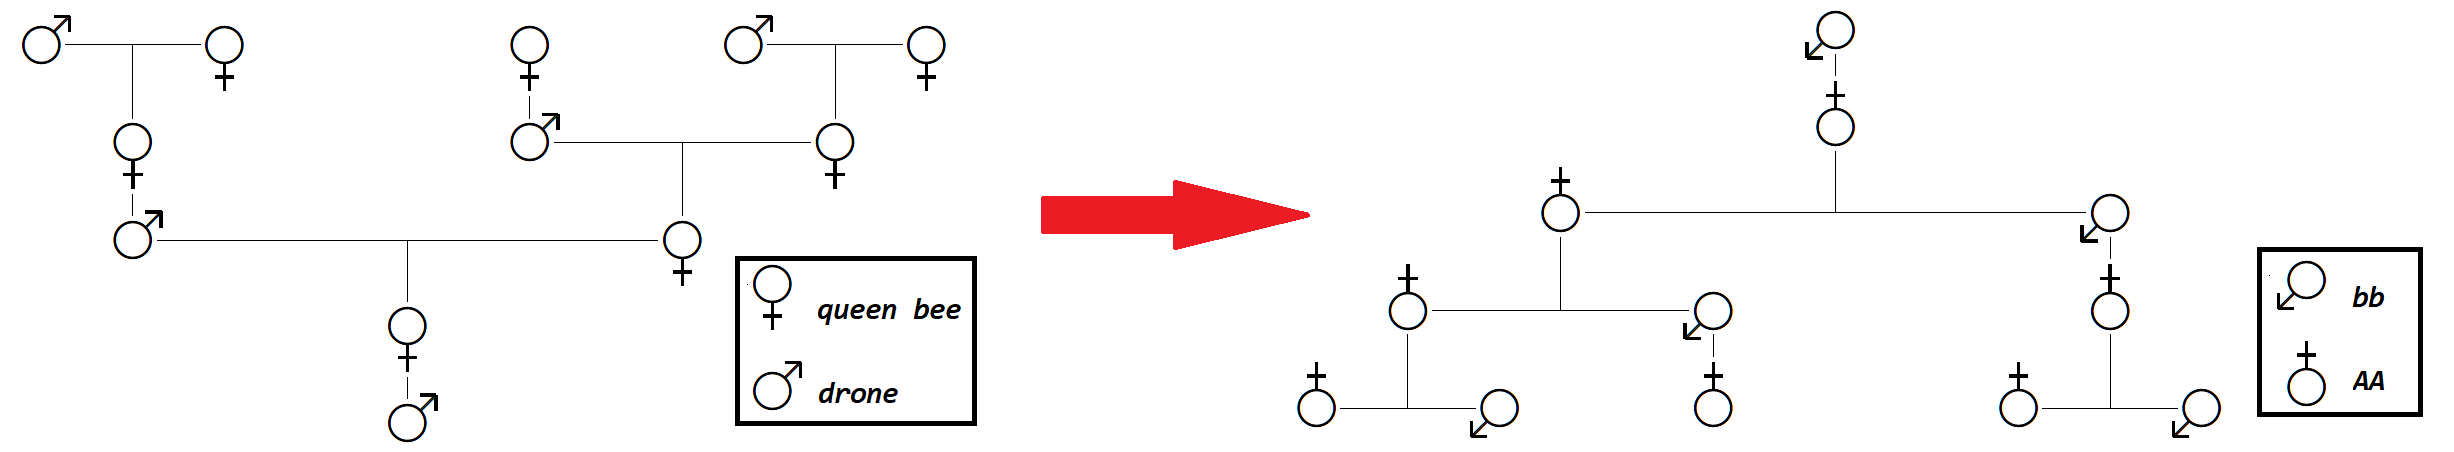
\includegraphics[width=6in]{6.png}\\
  \caption{The transformation from ``bee tree'' to ``rabbit tree''}\label{fig6}
\end{figure}

  Here are some brief explanations.
  \begin{itemize}
  \item Baby rabbits become adults after one month, which is represented as the vertical line from $bb$ to $AA$ in Figure \ref{fig6}.
  \item Each pair of adult rabbits produces one pair of baby rabbits every month, then there will be a pair of adult rabbits $AA$ and a pair of baby rabbits $bb$ a month later, which is represented as a fold line from $AA$ to $AA$ and $bb$ in Figure \ref{fig6}.
  \end{itemize}

  Since we know the conclusions of ``bee tree'', then we can easily derive the conclusions of our problem: $n$ month later, there will be $F_n$ pairs of adult rabbits and $F_{n-1}$ pairs of baby rabbits, where $F_n$ is the $n$-th element of Fibonacci Numbers. So there will be totally $F_n + F_{n-1} = F_{n+1}$ pairs of rabbits after $n$ months.
  \end{solution}

  \item [7. ] Show that Cassini's identity (6.103) is a special case of formula (6.108) in textbook, and a special case of formula (6.134) in textbook.
  \begin{solution}
  Let us denote $F_n$ as the $n$-th element of Fibonacci Numbers. The Cassini's identity (6.103) in textbook is as follows.
  \begin{displaymath}
  F_{n+1} F_{n-1} - F_n^2 = (-1)^n \qquad (n > 0)
  \end{displaymath}

  The formula (6.108) in textbook is as follows.
  \begin{displaymath}
  F_{n+k} = F_kF_{n+1} + F_{k-1}F_n
  \end{displaymath}

  Set $k$ as $(1-n)$ in the formula above and then we can derive the Cassini's identity (6.103).
  \begin{displaymath}
  \begin{aligned}
  &\quad F_{n + (1-n)} = F_{1-n} F_{n+1} + F_{1-n-1}F_n &\\
  \Longrightarrow &\quad F_1 = (-1)^{n-2} F_{n-1}F_{n+1} + (-1)^{n-1}F_n^2& \\
  \Longrightarrow &\quad F_{n+1} F_{n-1} - F_n^2 = (-1)^n &\qquad (n > 0)
  \end{aligned}
  \end{displaymath}

  Hence, Cassini's identity (6.103) is a special case of formula (6.108) in textbook.

  The formula (6.134) in textbook is as follows.

  \begin{displaymath}
  \begin{aligned}
    K_{m+n}(x_1,\cdots,x_{m+n})K_k(x_{m+1},\cdots,x_{m+k}) = & K_{m+k}(x_1,\cdots,x_{m+k})K_n(x_{m+1},\cdots,x_{m+n})\\
                                                             & + (-1)^k K_{m-1}(x_1,\cdots,x_{m-1})K_{n-k-1}(x_{m+k+2},\cdots,x_{m+n})
  \end{aligned}
  \end{displaymath}

  We already know that $K_n(1,\cdots,1) = F_{n+1}$, so we set $k$ as $(n-1)$, set $m$ as $1$ and set $x_1,x_2,\cdots$ as $1,1,\cdots$ in the formula above. Thus, we can derive the Cassini's identity (6.103).
  \begin{displaymath}
  \begin{aligned}
  & \quad F_{1+n+1} F_{(n-1)+1} = F_{(n-1)+1+1}F_n + (-1)^{n-1} F_{1-1+1}F_{n-(n-1)-1+1}&\\
  \Longrightarrow & \quad F_{n+2} F_n - F_{n+1}^2 = (-1)^{n-1}F_1^2 &\qquad (n \ge 0)\\
  \Longrightarrow & \quad F_{n+1} F_{n-1} - F_n^2 = (-1)^n &\qquad (n > 0)
  \end{aligned}
  \end{displaymath}
  Hence, Cassini's identity (6.103) is also a special case of formula (6.134) in textbook.
  \end{solution}

  \item [8. ] Use the Fibonacci system to convert $65 \textrm{\ mi/hr}$ into an approximate number of $\textrm{km/hr}$.
  \begin{solution}
  $65$ can be represented as $55 + 8 + 2$ in Fibonacci radix system. We can shift each number up one notch, getting $89 + 13 + 3 = 105$, which is the answer after unit transformation from $\textrm{mi/hr}$ to $\textrm{km/hr}$ according to the textbook. Then we know that $65 \textrm{\ mi/hr} \approx 105 \textrm{\ km/hr}$. The more precise answer is $104.61 \cdots$ and we can observe that our approximation is very close to the precise answer.
  \end{solution}
\end{enumerate}
\section{Basic Problems}
\begin{enumerate}
  \item [11. ] What is $\sum_k(-1)^k{n \brack m}$, the row sum of Stirling's cycle-number triangle with alternating signs, when $n$ is a nonnegative integer?
  \begin{solution}
  According to the general formula (6.11) in textbook, we can make the following derivations (Eqn.~\eqref{eq6}).
  \begin{equation}
  \sum_k {n \brack m} (-1)^k = (-1)^{\overline{n}} = \left\{
  \begin{aligned}
  & 1 & \qquad & (n = 0)\\
  & -1 & \qquad & (n = 1)\\
  & 0 & \qquad  & (n > 1)
  \end{aligned}\right. \quad \quad = [n=0] - [n=1]
  \label{eq6}
  \end{equation}
  \end{solution}

  \item [12. ] Prove that Stirling numbers have an inversion law analogous to Formula (5.48) in textbook:
  \begin{displaymath}
  g(n) = \sum_k {n \brace k} (-1)^k f(k) \quad \Longleftrightarrow \quad f(n) = \sum_k {n \brack k} (-1)^k g(k)
  \end{displaymath}
  \begin{proof} We can split the conclusion to two sub-conclusions and prove them respectively.
  \begin{itemize}
  \item \textbf{($\Longrightarrow$)} If we have $g(n) = \sum_k {n \brace k} (-1)^k f(k)$, then $f(n) = \sum_k {n \brack k} (-1)^k g(k)$ is correct.
  \begin{displaymath}
  \begin{aligned}
  f(n) &= \sum_k{ {n \brack k} (-1)^k g(k)} \\
       &= \sum_k{{n \brack k} (-1)^k \left(\sum_m {{k \brace m} (-1)^m f(m)} \right)} \\
       &= \sum_m{\sum_k {{n \brack k} {k \brace m} (-1)^{k+m} f(m)}} \\
       &= \sum_m{(-1)^{n+m}f(m)\sum_k {{n \brack k} {k \brace m} (-1)^{n-k}}} \\
       &= \sum_m{(-1)^{n+m}f(m)[m=n]} \\
       &= f(n)
  \end{aligned}
  \end{displaymath}
  Notice that we use an important formula (6.31) in textbook in the derivations. Therefore, the correctness is proved.
  \item \textbf{($\Longleftarrow$)} If we have $f(n) = \sum_k {n \brack k} (-1)^k g(k)$, then $g(n) = \sum_k {n \brace k} (-1)^k f(k)$ is correct. The proof process is similar to the previous one and we can come to the similar result that the conclusion is correct.
  \end{itemize}
  Therefore, the conclusion is correct.
  \end{proof}

  \item [13. ] The differential operators $\mathrm{D} = \frac{\mathrm{d}}{\mathrm{d}z}$ and $\vartheta = z\mathrm{D}$ are mentioned in Chapters 2 and 5. We have
  \begin{displaymath}
  \vartheta^2 = z^2\mathrm{D}^2 + z\mathrm{D}
  \end{displaymath}
  because $\vartheta^2 f(z) = \vartheta z f'(z) = z\frac{\mathrm{d}}{\mathrm{d}z}zf'(z) = z^2 f''(z) + zf'(z)$, which is $(z^2\mathrm{D}^2+z\mathrm{D})f(z)$. Similarly it can be shown that $\vartheta^3 = z^3\mathrm{D}^3 + 3z^2\mathrm{D}^2 + z\mathrm{D}$. Prove the general formulas for all $n \ge 0$.
  \begin{displaymath}
  \begin{aligned}
  \vartheta^n &= \sum_k {n \brace k} z^k \mathrm{D}^k \\
  z^n \mathrm{D}^n &= \sum_k {n \brack k} (-1)^{n-k} \vartheta^k
  \end{aligned}
  \end{displaymath}
  (These can be used to convert between differential expressions of the forms $\sum_k \alpha_kz^kf^{(k)}(z)$ and $\sum_k \beta_k\vartheta^kf(z)$, as in (5.109).)
  \begin{proof}
  Let us prove the former formula (i.e., $\vartheta^n = \sum_k {n \brace k} z^k \mathrm{D}^k$) first by induction on $n$.
  \begin{itemize}
  \item \textbf{(Induction Basis)} When $n = 0$, the conclusion is obviously true, since $\vartheta^0 = \mathrm{I}$ and $\sum_k {0 \brace k} z^k \mathrm{D}^k = \mathrm{I}$, where $\mathrm{I}$ is an identity operator.
  \item \textbf{(Induction Step)} Suppose the formula is true for $n = m$, that is, $\vartheta^m = \sum_k {m \brace k} z^k \mathrm{D}^k$. We are going to prove that the formula still holds for $n = m+1$. Let us make some simple derivations first (Eqn.~\eqref{eq131}).
      \begin{equation}
      \vartheta^{m+1} = \vartheta(\vartheta^m) = \vartheta\left(\sum_k {m \brace k} z^k \mathrm{D}^k\right) = \sum_k {m \brace k} \vartheta(z^k \mathrm{D}^k)
      \label{eq131}
      \end{equation}

      We know that $\vartheta(z^k \mathrm{D}^k) = z\mathrm{D}(z^k \mathrm{D}^k) = z(z^k D^{k+1} + kz^{k-1}D^k) = z^{k+1}D^{k+1} + kz^kD^k$. Plug this result in the Equation \eqref{eq131}, we can make the following derivations.

      \begin{displaymath}
      \begin{aligned}
      \vartheta^{m+1} & = \sum_k {m \brace k} (z^{k+1}D^{k+1} + kz^kD^k) \\
                      & = \sum_k k {m \brace k} z^k D^k + \sum_k {m \brace k-1} z^k D^k \\
                      & = \sum_k \left(k {m \brace k} + {m \brace k-1}\right)z^kD^k \\
                      & = \sum_k {m + 1 \brace k} z^kD^k
      \end{aligned}
      \end{displaymath}
      Hence, the conclusion holds for $n = m+1$.
  \end{itemize}
  In summary, the former formula (i.e., $\vartheta^n = \sum_k {n \brace k} z^k \mathrm{D}^k$) is proved, then we are going to use it to derive the latter formula (i.e., $z^n \mathrm{D}^n = \sum_k {n \brack k} (-1)^{n-k} \vartheta^k$).

  According to the inversion law of Stirling's Number that we have proved in problem 12 before, we know that for any two function $f(\cdot), g(\cdot)$, we have
  \begin{displaymath}
  g(n) = \sum_k {n \brace k} (-1)^k f(k) \quad \Longleftrightarrow \quad f(n) = \sum_k {n \brack k} (-1)^k g(k)
  \end{displaymath}

  This is still correct for any two operators $\mathrm{F}_i, \mathrm{G}_i$, that is,
  \begin{displaymath}
  \mathrm{G}_n = \sum_k {n \brace k} (-1)^k \mathrm{F}_k \quad \Longleftrightarrow \quad \mathrm{F}_n = \sum_k {n \brack k} (-1)^k \mathrm{G}_k
  \end{displaymath}

  We set $\mathrm{G}_n$ as $\vartheta^n$ and set $\mathrm{F}_n$ as $(-1)^nz^n\mathrm{D}^n$. Thus, we can transform our former formula to the following formula.
  \begin{displaymath}
  \mathrm{G}_n = \sum_k {n \brace k} (-1)^k \mathrm{F}_k
  \end{displaymath}

  According to the inversion law of Stirling's Number for operators that we have stated before, we can come to the following conclusion.
  \begin{displaymath}
  \mathrm{F}_n = \sum_k {n \brack k} (-1)^k \mathrm{G}_k
  \end{displaymath}

  Unfold notations $\mathrm{F}_i$ and $\mathrm{G}_i$, we can derive our latter formula.
  \begin{displaymath}
  (-1)^nz^n\mathrm{D}^n = \sum_k {n \brack k} (-1)^k \vartheta^k \quad \Longrightarrow \quad z^n\mathrm{D}^n = \sum_k {n \brack k} (-1)^{n-k} \vartheta^k
  \end{displaymath}
  Hence, we have proved the latter formula using the former formula and the inversion law of Stirling's Number. In conclusion, two formulas are correct.
  \end{proof}
\end{enumerate}
%=================== =====================================================
\end{document}
